\documentclass[dvipdfmx]{jsarticle}
\usepackage[dvipdfmx]{graphicx}
\usepackage{amsmath, amssymb}
\usepackage{mathtools}
\usepackage{here}
\usepackage{listings}

\lstset{
  basicstyle={\ttfamily},
  identifierstyle={\small},
  commentstyle={\smallitshape},
  keywordstyle={\small\bfseries},
  ndkeywordstyle={\small},
  stringstyle={\small\ttfamily},
  frame={tb},
  breaklines=true,
  columns=[l]{fullflexible},
  numbers=left,
  xrightmargin=0zw,
  xleftmargin=3zw,
  numberstyle={\scriptsize},
  stepnumber=1,
  numbersep=1zw,
  lineskip=-0.5ex
}

\renewcommand{\lstlistingname}{ソースコード}

\renewcommand{\thefigure}{\thesection-\arabic{figure}}
\setcounter{section}{5}
\setcounter{figure}{17}

\begin{document}

\section*{5.5 活性化関数レイヤの実装}
この節では,計算グラフの考え方をニューラルネットワークに適用する.ここでは,ニューラルネットワークを構成する「層(レイヤ)」をひとつのクラスとして実装する.まずは,活性化関数であるReLUとSigmoidレイヤを実装する.

\section*{5.5.1 ReLUレイヤ}
活性化関数として使われるReLU(Rectified Linear Unit)は,次の式(5.7)で表された.

\begin{equation}
y =
\begin{dcases}
x & (x > 0) \\
0 & (x \leqq 0)
\end{dcases}
\tag{5.7}
\end{equation}

式(5.7)から,$x$に関する$y$の微分は式(5.8)のように求められる.計算グラフで表すと,図5-18のように書くことができる.

\begin{equation}
    \frac{\partial y}{\partial x} =
    \begin{dcases}
    1 & (x > 0) \\
    0 & (x \leqq 0)
    \end{dcases}
\tag{5.8}
\end{equation}

\begin{figure}[htbp]
\begin{center}
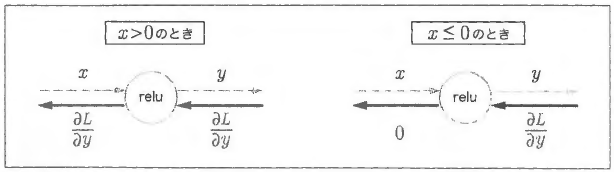
\includegraphics[width=0.9\linewidth]{./spring_lec/DL5-5-1.png}
\end{center}
\caption{ReLUレイヤの計算グラフ}
\end{figure}

では,このReLUレイヤの実装を行う.実装は,以下のソースコードのようになる.

\begin{lstlisting}[caption=ReLU,label=fuga]
class Relu:
    def __init__(self):
        self.mask = None

    def forward(self, x):
        self.mask = (x <= 0)
        out = x.copy()
        out(self.mask) = 0

        return out
    
    def backward(self, dout):
        dout[self.mask] = 0
        dx = dout

        return dx
\end{lstlisting}


Reluクラスは,maskというインスタンス変数を持つ.maskは,True/FalseからなるNumpy配列で,順伝播の入力であるxの要素で0以下の場所をTrue,0より大きい要素をFalseとして保持する.

\begin{lstlisting}[caption=maskの例, label=fuga]
>>> x = np.array([[1.0, -0.5], [-2.0, 3.0]])
>>> print(x)
[[ 1. -0.5]
 [-2.  3. ]]
>>> mask = (x <= 0)
>>> print(mask)
[[False True]
 [True False]]
\end{lstlisting}

図5-18に示すように,順伝播の入力が0以下ならば,逆伝播の値は0になるため,逆伝播では,順伝播時に保持したmaskを用いて,上流から伝播されたdoutに対して,maskの要素がTrueの場所を0に設定する.

\section*{5.5.2 Sigmoidレイヤ}
続いて,シグモイド関数を実装する.シグモイド関数を計算グラフで表すと,次の図5-19のようになる.

\begin{figure}[H]
\begin{center}
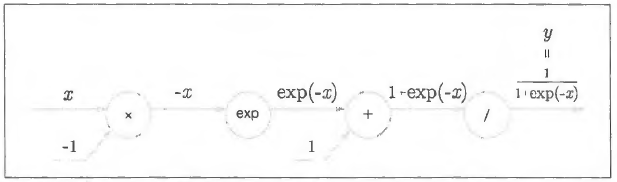
\includegraphics[width=0.9\linewidth]{./spring_lec/DL5-5-2.png}
\end{center}
\caption{Sigmoidレイヤの計算グラフ(順伝播のみ)}
\end{figure}

図5-19では「×」と「+」ノードの他に,「exp」と「/」ノードが新しく登場している.「exp」ノードは$y = \exp(x)$の計算を行い,「/」ノードは,$y = \frac{1}{x}$の計算をする.
Sigmoidレイヤの逆伝播の計算の流れをまとめると,図5-20のような計算グラフとなる.

\begin{figure}[H]
\begin{center}
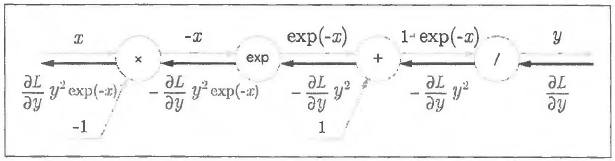
\includegraphics[width=0.9\linewidth]{./spring_lec/DL5-5-3.png}
\end{center}
\caption{Sigmoidレイヤの計算グラフ}
\end{figure}

図5-20の結果から逆伝播の出力は,$\frac{\partial L}{\partial y} y^2 \exp(-x)$となり,この値が下流にあるノードに伝播していく.ここで$\frac{\partial L}{\partial y} y^2 \exp(-x)$という値が順伝播の入力$x$と出力$y$だけから計算できる点に注目すると,次の図5-21のようなグループ化した「sigmoid」ノードとして書くことができる.

そして,$\frac{\partial L}{\partial y} y^2 \exp(-x)$は,さらに次のように整理して書くことができる.
\begin{align}\label{}
\notag
\frac{\partial L}{\partial y} y^2 \exp(-x) &= \frac{\partial L}{\partial y} \frac{1}{(1 + \exp(-x))^2} \exp(-x) \\
&= \frac{\partial L}{\partial y} \frac{1}{1 + \exp(-x)} \frac{\exp(-x)}{1 + \exp(-x)} \tag{5.12} \\
&= \frac{\partial L}{\partial y} y(1 - y) \notag
\end{align}

そのため,図5-21で表されるSigmoidレイヤの逆伝播は,順伝播の出力だけから計算することが出来る.

\begin{figure}[htbp]
\begin{center}
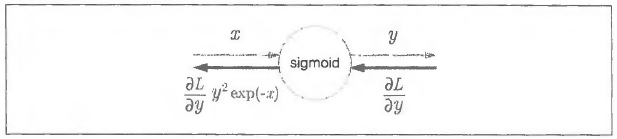
\includegraphics[width=0.9\linewidth]{./spring_lec/DL5-5-4.png}
\end{center}
\caption{Sigmoidレイヤの計算グラフ:順伝播の出力$y$によって,逆伝播の計算を行うことができる}
\end{figure}

\begin{lstlisting}[caption=Sigmoid, label=fuga]
class Sigmoid:
    def __init__(self):
        self.out = None
    def forward(self, x):
        out = 1 / (1 + np.exp(-x))
        self.out = out

        return out
    
    def backward(self, dout):
        dx = dout * (1.0 - self.out) * self.out

        return dx
\end{lstlisting}


この実装では,順伝播時に出力をインスタンス変数のoutに保持している.そして逆伝播時に,そのout変数を使って計算を行う.

\end{document}